\section{Zielsetzung}
\label{sec:ziel}

Ziel des Versuchs ist es, quantenmechanische Strukturen wie das Wasserstoffatom, Wasserstoffmolekül und die Bandstruktur in eindimensionalen Festkörpern mit Hilfe von Analogien in der Akustik zu untersuchen und die Gemeinsamkeiten und Grenzen dieser Analogien zu untersuchen. Dazu werden akustische Experimente mit Hohlraumresonatoren und Zylindern aus Aluminium durchgeführt.

\section{Theorie}
\label{sec:theorie}

Für die quantenmechanischen Modellen können Analogien mit Hilfe der Akustik geschaffen werden, im Folgenden werden die quantenmechanischen Grundlagen für die einzelnen Modelle erläutert und die Gemeinsamkeiten und Unterschiede zu den akustischen Experimenten benannt und begründet. 

\subsection{Das Wasserstoffatom}
\label{sec:H}

Das Wasserstoffatom ist das simpelste Atom. Es besteht aus einem Proton im Kern und einem Elektron in der Hülle. Die zeitunabhängige Schrödingergleichung für dieses System lautet:

\begin{equation}
    \hat{H} \, \Psi \! \left( \vec{r} \right) = - \frac{\hbar^2}{2 m} \! \Laplace \, \Psi \! \left( \vec{r} \right)- \frac{e^2}{4 \pi \epsilon_0 r} \, \Psi \! \left( \vec{r} \right) = E \, \Psi \! \left( \vec{r} \right)
    \label{eqn:schroedinger}
\end{equation}

Dabei ist $\Psi \! \left( \vec{r} \right)$ ist die Wellenfunktion, $E$ die Gesamtenergie und $\hat{H}$ der Hamiltonoperator. Für ein Elektron im Wasserstoffatom lautet $\hat{H}$:

\begin{equation}
    \hat{H} = - \frac{\hat{p}^2}{2 m} - \frac{e^2}{4 \pi \epsilon_0 r}
    \label{eqn:H_H}
\end{equation}

Hierbei ist $\hat{p}$ der Impulsoperator, $\hbar$ das gekürzte Planksche Wirkungsquantum, $m$ die Masse des Elektrons, $e$ die Elementarladung und $\epsilon_0$ die elektrische Feldkonstante. Aufgrund der Kugelsymmetrie des Systems werden Kugelkoordinaten verwendet, dort lautet der Laplace-Operator $\Laplace$:

\begin{equation}
    \Laplace = \frac{1}{r^2} \frac{\partial}{\partial r} \left( r^2 \frac{\partial}{\partial r} \right) + \frac{1}{r^2 \sin \theta} \frac{\partial}{\partial \theta} \left( \sin \theta \frac{\partial}{\partial \theta} \right) + \frac{1}{r^2 \sin^2 \theta} \frac{\partial^2}{\partial \varphi^2} = \Laplace_r + \frac{1}{r^2} \Laplace_{\theta, \varphi}
    \label{eqn:laplace}
\end{equation}

Um die Schrödingergleichung zu lösen wird die Wellenfunktion $\Psi$ mit dem Separationsansatz in einen Radialteil $R_{nl}$ und einen Winkelanteil $\Phi_{lm}$ aufgeteilt:

\begin{equation}
    \Psi_{nlm} (\vec{r}) = R_{nl}(r) \, \Phi_{lm}(\theta, \varphi)
    \label{eqn:seperation}
\end{equation}

Für das Wasserstoffatom gibt es 3 Quantenzahlen namens $n, l, m$. Dabei ist $n$ die Hauptquantenzahl, $l$ die Nebenquantenzahl und $m$ die Magnetquantenzahl. Für die Quantenzahlen gilt

\begin{align*}
    n &\in \mathbb{N} \\
    l &\in \mathbb{N}_0 \\
    m &\in \mathbb{Z}
\end{align*}

und

\begin{align*}
    l &< n \\
    |m| &\leq l .
\end{align*}

Mit dem Separationsansatz entstehen zwei entkoppelte Differentialgleichungen. Für dieses Experiment ist jedoch nur die Lösung des Winkelanteils interessant, da nur dieser in dem akustischen Modell modelliert werden kann. Dies führt für den Radialanteil und Winkelanteil zu folgender Differentialgleichung:

\begin{align}
    E R_{nl}(r) &= \left( - \frac{\hbar^2}{2mr} \frac{\partial^2}{\partial r^2} r - \frac{\hbar^2}{2mr^2} l(l+1) - \frac{e^2}{r} \right) R_{nl}(r)
    \label{eqn:radial_DGL} \\
    - l (l+1) \Phi_{lm} &= \Laplace_{\theta, \varphi} \, \Phi_{lm} (\theta, \varphi) 
    \label{eqn:winkel_DGL}
\end{align}

Dabei ist $\Laplace_{\theta, \varphi}$ der Winkelanteil des Laplaceoperators $\Laplace$ in Kugelkoordinaten. Der Term mit $l (l+1)$ kommt in der Herleitung dadurch zustande, dass $- \hbar^2 \Laplace_{\theta, \varphi} = \hat{L}^2$ entspricht, wobei $\hat{L}$ der Drehimpulsoperator ist. Für $\hat{L}^2$ gilt folgende Eigenwertgleichung:

\begin{equation}
    \hat{L}^2 \ket{\psi} = \hbar^2 l(l+1) \ket{\psi}
    \label{eqn:L}
\end{equation}

Die Eigenwertgleichung \eqref{eqn:winkel_DGL} kann mit Hilfe der \textit{Kugelflächenfunktionen} $Y_{lm} (\theta, \varphi)$ gelöst werden und diese ergeben sich zu:

\begin{equation}
    Y_{lm} (\theta, \varphi) = \frac{1}{\sqrt{2 \pi}} N_{lm} P_{lm} (\cos \theta) e^{im \varphi}
    \label{eqn:kugelflaechen}
\end{equation}

Hierbei bezeichnet $P_{lm}$ die zugeordneten \textit{Legendrepolynome}

\begin{equation}
    P_{lm} (x) = \frac{(-1)^m}{2^l \, l!} \left( 1-x^2 \right)^{\! \frac{m}{2}} \frac{d^{\, l+m}}{dx^{l+m}} \left( x^2 - 1 \right)^l
    \label{eqn:legendre}
\end{equation}

und $N_{lm}$ den Normierungsfaktor

\begin{equation}
    N_{lm} = \sqrt{\frac{2 \, l +1}{2} \cdot \frac{(l-m)!}{(l+m)!}} .
    \label{eqn:normierung}
\end{equation}

Die Eigenenergiewerte des Wasserstoffatoms betragen:

\begin{equation}
    E_n = - \frac{e^2}{8 \pi \epsilon_0 a_0} \cdot \frac{1}{n^2}
    \label{eqn:H_energien}
\end{equation}

Dabei bezeichnet $a_0 = \frac{4 \pi \epsilon_0 \hbar^2}{m e^2}$ den Bohrschen Radius. In Gleichung \eqref{eqn:H_energien} ist auffällig, dass die Eigenenergiewerte beim Wasserstoffatom eine Entartung in $m$ aufzeigen, die durch die sphärische Symmetrie resultiert. Diese Entartung kann durch ein Anlegen eines äußeren Magnetfeldes aufgehoben werden. Durch die Felder wird die Symmetrie gebrochen. Dieser Effekt wird \textit{Zeemanneffekt} genannt. Die Entartung in $l$ ist jedoch ein Resultat aus dem $\nicefrac{1}{r}$ - Potential. Zusätzlich führt die Berücksichtigung von Spin und relativistischen Beiträgen zu weiteren Aufspaltungen, diese wurden hierbei jedoch nicht berücksichtigt.

\subsection{Das Wasserstoffmolekül}
\label{sec:H2}

Das Wasserstoffmolekül $H_2$ besteht aus 2 Wasserstoffatomen und ist damit das einfachste neutrale Molekül. Es besteht also aus 2 positiven Protonen und 2 Elektronen. Dieses Problem ist jedoch nicht analytisch lösbar. Jedoch existieren Näherungen, um die Wellenfunktion des Systems zu approximieren. Die zu lösende Schrödingergleichung lautet:

\begin{equation}
    E \, \Psi (1, 2) = \left( \hat{H}_1 + \hat{H}_2 - \frac{e^2}{r_{a2}} - \frac{e^2}{r_{b1}} - \frac{e^2}{r_{12}} - \frac{e^2}{R_{ab}} \right) \, \Psi (1, 2)
    \label{eqn:H2}
\end{equation}

Hierbei sind $\hat{H}_{1,2}$ die Hamiltonoperatoren der einzelnen Wasserstoffatome, und die anderen Variablen beschreiben die Abstände der Elektronen 1 und 2 zu den Kernen a und b aus Abbildung \ref{fig:H2}.

\begin{figure}[H]
    \centering
    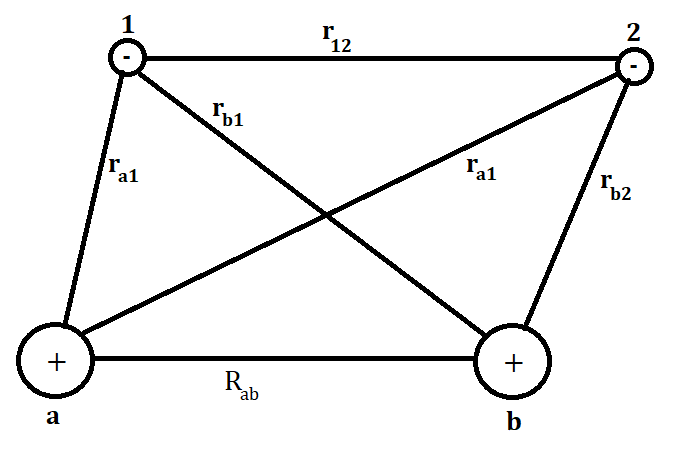
\includegraphics[width=0.7\textwidth]{H2.PNG}
    \caption{Schematische Skizze des Wasserstoffmoleküls.}
    \label{fig:H2}
\end{figure}

Da die Elektronen Fermionen sind unterliegen sie dem \textit{Pauli-Verbot} und dies muss auch die Wellenfunktion erfüllen. Also muss die Gesamtwellenfunktion antisymmetrisch sein. Die Gesamtwellenfunktion $\Psi (1,2)$ besteht aus einer Ortswellenfunktion $\tilde{\Psi} (1,2)$ und einer Spinwellenfunktion $S (1,2)$:

\begin{equation}
    \Psi (1,2) = \tilde{\Psi} (1,2) \cdot S (1,2)
    \label{eqn:gesamt}
\end{equation}

Dadurch muss die Spinwellenfunktion antisymmetrisch sein, falls die Ortswellenfunktion symmetrisch ist und vice versa. Dadurch ergeben sich 4 mögliche Wellenfunktionen:

\begin{align}
    \Psi_{t1} (r_1, r_2) &= \, \uparrow_1 \uparrow_2 \left( \Psi_a (r_1) \Psi_b (r_2) - \Psi_a (r_2) \Psi_b (r_1) \right) \label{eqn:wellenfunktion1}\\
    \Psi_{t2} (r_1, r_2) &= \, \downarrow_1 \downarrow_2 \left( \Psi_a (r_1) \Psi_b (r_2) - \Psi_a (r_2) \Psi_b (r_1) \right) \\
    \Psi_{t3} (r_1, r_2) &= \frac{1}{\sqrt{2}} \left( \uparrow_1 \downarrow_2 + \uparrow_2 \downarrow_1 \right) \left( \Psi_a (r_1) \Psi_b (r_2) - \Psi_a (r_2) \Psi_b (r_1) \right) \\
    \Psi_{s} (r_1, r_2) &= \frac{1}{\sqrt{2}} \left( \uparrow_1 \downarrow_2 - \uparrow_2 \downarrow_1 \right) \left( \Psi_a (r_1) \Psi_b (r_2) + \Psi_a (r_2) \Psi_b (r_1) \right)
    \label{eqn:wellenfunktion4}
\end{align}

Hierbei bezeichnet $\uparrow_i$ und $\downarrow_i$ den jeweiligen Spin des jeweiligen Elektrons und $r_i$ bezeichnet die Position im Raum des Elektrons. Dabei bilden die $\Psi_t$ Wellenfunktionen das \textit{Triplett} mit antisymmetrischer Ortswellenfunktion und symmetrischer Spinwellenfunktion, dies wird als \textit{Orthowasserstoff} bezeichnet. $\Psi_s$ ist das \textit{Singulett} mit antisymmetrischer Spinwellenfunktion und symmetrischer Ortswellenfunktion und wird als \textit{Parawasserstoff} bezeichnet. Beim Wasserstoffmolekül gibt es \textit{bindende} und \textit{anti-bindende Zustände}, diese werden durch den Phasenunterschied $\increment \varphi$ definiert. Nur bei einer Überlappung mit einem geraden Zustand, wirkt das Resultat bindend und bei einem Phasenunterschied von $\increment \varphi = \pi$ wird dieser Zustand als ungerade bezeichnet und wirkt antibindend.

\subsection{Der 1-dim Festkörper}
\label{sec:festkoerper}

Beim Festkörper kommt es durch das Pauli-Prinzip, nachdem 2 Fermionen wie Elektronen sich nicht gleichzeitig im selben Zustand befinden dürfen, im Gegensatz zum Wasserstoffatom nicht zu scharfen Spektrallinien, sondern zu Energiebändern, die aus den \textit{erlaubten Zonen} bestehen. Zwischen den Energiebändern gibt es Bandlücken, die aus den \textit{verbotenen Zonen} bestehen. Um einen Festkörper zu modellieren werden Kastenpotentiale mit periodischen Randbedingungen verwendet. Dadurch ergibt sich in der Dispersionsrelation $E(\vec{k})$ in erster Näherung eine Proportionalität zu $k^2$. Die Dispersionsrelation beträgt:

\begin{equation}
    E(k) = \frac{\hbar^2 k^2}{2 m}
    \label{eqn:disp}
\end{equation}

In einem eindimensionalen Festkörper wird ein Elektron in einem periodischen Potential $U(x)$ betrachtet. Das Potential und die Wellenfunktion in eine Fourierreihe entwickelt ergibt dann:

\begin{align}
    U (x) &= \sum_G U_G \cdot e^{iGx} \\
    \Psi (x) &= \sum_k C_k \cdot e^{ikx}
\end{align}

Aus den periodischen Randbedingungen ergibt sich dann $k = \frac{2 \pi}{L} n$. Dies eingesetzt in die Schrödingergleichung ergibt dann:

\begin{equation}
    E \, \Psi (x) = \left( - \frac{\hbar^2}{2m} \Laplace + U (x) \right) \Psi (x)
    \label{eqn:fest_schroed}
\end{equation}

Für ein Elektron ergibt sich dann folgende Gleichung:

\begin{equation}
    \left( \frac{\hbar^2 k^2}{2m} - E \right) C_k + \sum_G U_G C_{k-G} = 0
    \label{eqn:fest_el}
\end{equation}

Die Darstellung der Dispersionsrelation muss jedoch auf ein reduziertes Zonenschema mit Wellenvektor beschränkt auf $- \nicefrac{\pi}{a} \leq k \leq \nicefrac{\pi}{a}$ eingegrenzt werden. Das vollständige Zonenschema ergibt sich durch periodisches aneinander Reihen dieser Dispersionsrelation vom reduzierten Zonenschema. Die Zone, die das reduzierte Zonenschema umfasst, wird auch als die \textit{erste Brillouin-Zone} bezeichnet.

Jedoch sind Festkörper in der Realität nicht zu $100 \%$ reine Kristalle und besitzen oft Defekte. Diese Defekte werden häufig durch Fehlstellen oder Fremdatome in der Kristallstruktur ausgelöst und müssen durch veränderte Potentialtöpfe modelliert werden.

\subsection{Analogie zum Wasserstoffatom und -molekül}
\label{sec:analogien}

Im Folgenden werden die Analogien zwischen akustischen Experimenten und dem Modell des Wasserstoffatoms und Wasserstoffmolekül dargestellt. 

\subsubsection{Wasserstoffatom}
\label{sec:ana-H}

Für einen Kugelresonator gilt im klassischen Fall die Helmholtzgleichung mit

\begin{equation}
    \frac{\partial^2 p(\vec{r}, t)}{\partial t^2} = \frac{\Laplace p(\vec{r}, t)}{\rho \kappa} ,
    \label{eqn:helmholtz}
\end{equation}

wobei $p(\vec{r}, t)$ der Druck ist an der Stelle $\vec{r}$ zur Zeit $t$, $\rho$ und $\kappa$ sind dabei die Dichte und die Kompressibilität des Mediums bzw. der Luft. Ähnlich wie im quantenmechanischen Modell lässt sich die Zeitentwicklung von der räumlichen Entwicklung separieren, dafür wird folgender Ansatz verwendet:

\begin{equation}
    p(\vec{r}, t) = p(\vec{r}) \cdot \cos(\omega t)
    \label{eqn:akus_sep}
\end{equation}

Durch Einsetzen von $\nicefrac{1}{c^2} = \rho \kappa$, wobei $c$ die Schallgeschwindigkeit ist, ergibt sich die stationäre Druckverteilung mit dem Laplaceoperator $\Laplace$ aus Gleichung \eqref{eqn:laplace} in Kugelkoordinaten:

\begin{equation}
    - \frac{\omega^2}{c^2} p(\vec{r}) = \Laplace p(\vec{r}) = \left( \Laplace_r + \frac{1}{r^2} \Laplace_{\theta, \varphi} \right) p(\vec{r})
    \label{eqn:stationaer}
\end{equation}

Äquivalent wie in Kapitel \ref{sec:H} kann dieses Problem durch Separation mit $p(r, \theta, \varphi) = \Psi_{lm}(\theta, \varphi) \cdot R(r)$ in einen Radial- und Winkelanteil separiert werden und es entstehen 2 unabhängige Gleichungen:

\begin{align}
    -l(l+1) \Psi_{lm} (\theta, \varphi) &= \Laplace_{\theta, \varphi} \, \Psi_{lm} (\theta, \varphi)
    \label{eqn:akus_winkel} \\
    \frac{\omega^2}{c^2} R(r) &= \left( - \frac{\partial^2}{\partial r^2} - \frac{2}{r} \frac{\partial}{\partial r} + \frac{l(l+1)}{r^2} \right) R(r)
    \label{eqn:akus_raeumlich}
\end{align}

Der Vergleich zwischen der DGL \eqref{eqn:winkel_DGL} beim Wasserstoffatom und der DGL \eqref{eqn:akus_winkel} beim Kugelresonator zeigt, dass sie identisch sind. Lediglich die DGL \eqref{eqn:akus_raeumlich} für den radialen Anteil ist unterschiedlich zu der DGL \eqref{eqn:radial_DGL} für den radialen Anteil vom Wasserstoffatom. Dadurch besteht keine Analogie zum radialen Anteil zwischen dem klassischen Modell und dem quantenmechanischen, dafür kann der Winkelanteil im klassischen Modell als Analogie zum quantenmechanischen benutzt werden. Im Kugelresonator treten dann beim Einschalten des Lautsprechers Resonanzfrequenzen auf, die mit dem Mikrofon vermessen werden können. Im Wasserstoffatom tritt sowohl eine Entartung in $l$ als auch eine $2l+1$ -fache Entartung in $m$ auf. Im klassischen Kugelresonator wird die Entartung in $l$ nicht realisiert, da dort kein $\nicefrac{1}{r}$ -Potential vorherrscht. Die Entartung von $m$ existiert jedoch auch im klassischen Analogon. Im Wasserstoffatom könnte die Entartung durch Anlegen eines Magnetfeldes und den dadurch entstehenden \textit{Zeeman-Effekt} aufgehoben werden, im Kugelresonator geschieht dies durch Symmetriebrechung. Ein schematischer Aufbau des Hohlresonators ist in Abbildung \ref{fig:modell} zu sehen.

\begin{figure}[H]
    \centering
    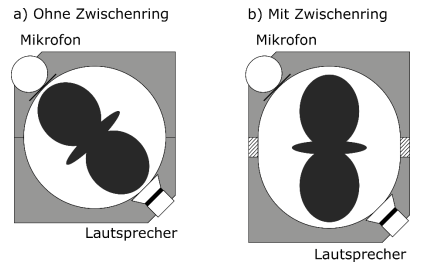
\includegraphics[width=0.8\textwidth]{Skizze.PNG}
    \caption{Schematischer Aufbau des Kugelresonators. \cite{Anleitung}}
    \label{fig:modell}
\end{figure}

Ohne den Zwischenring wird durch die Stellung von Mikrofon und Lautsprecher und die Symmetrie derer nur die $m=0$ Moden angeregt. Durch Einsetzen eines Zwischenrings wie in Abbildung \ref{fig:modell} wird die Symmetrie gebrochen und es werden nun auch die $m \neq 0$ Moden angeregt. Dadurch wird die Entartung in $m$ teilweise aufgehoben. Dabei sind durch den Zwischenring nur noch die jeweiligen $+m$- und $-m$-Moden entartet. Die Kugelflächenfunktionen sind nun durch die Zwischenringe eigentlich auch keine exakten Lösungen mehr, aber sie sind immer noch näherungsweise eine Lösung des Systems. Im Allgemeinen ergeben die Messungen mit dem Mikrofon in der Analogie auch nur das Betragsquadrat $|\Psi|^2$ der Wellenfunktion und nicht die Wellenfunktion $\Psi$ an sich.

\subsubsection{Wasserstoffmolekül}
\label{sec:ana-H2}

Für das Wasserstoffmolekül werden zwei Kugelresonator über eine kreisförmige Blende miteinander verbunden. Genau wie im Wasserstoffmolekül sind die Wellenfunktionen der einzelnen Elektronen bzw. den einzelnen Kugelresonatoren miteinander gekoppelt und verbunden. Die dabei entstehenden Orbitale überlappen dann in den verbundenen Resonatoren. Genau wie beim Wasserstoffmolekül gibt es \textit{bindende} und \textit{anti-bindende Zustände}, diese werden auch über den Phasenunterschied $\increment \varphi$ definiert wie im Ende von Abschnitt \ref{sec:H2} beschrieben.

\subsection{Analogie zum 1-dim Festkörpers}
\label{ana-fest}

Beim akustischen Analogon werden Aluminiumzylinder mit Irisblenden zu einer linearen Kette gereiht. Für einen zylindrischen Hohlraumresonator ist die Dispersionsrelation linear abhängig zur Wellenzahl $\kappa$, im Festkörper ist ein quadratischer Zusammenhang vorhanden. Resonanzen entstehen, wenn die Länge des Zylinders einem Vielfachen der Wellenlänge des Schalls entspricht. Die einzelnen Röhren werden mit Blenden aneinander gereiht, dadurch beeinflussen sich die einzelnen Resonatoren gegenseitig. Die Strecke von einer Blende zur nächsten entspricht im akustischen Analogon der ersten Brillouin-Zone. Der Durchmesser der Öffnungen der eingesetzten Blenden entspricht dann der Kopplungsstärke der einzelnen Resonatoren und jede Schallwelle wird beim Durchlaufen der Blende gestreut. Defekte stören die Periodizität in einem reellen Festkörper, im Akustikexperiment werden die Störungen durch einzelne Zylinder in der Kette simuliert, die entweder kürzer oder länger sind als die anderen. Dadurch entstehen Störungen in der Resonatorkette und diese können als Defekte bezeichnet werden.